%\section{Training a Sentence Classifier without Alignment \label{sec:uschema}}
\section{Methods \label{sec:methods}}

\subsection {Universal Schema}

\begin{figure}[h]
\caption{Universal schema represents relation types and entity pairs as a matrix.
1's are observed training examples and the bolded .93 is predicted by the model.}
\centering
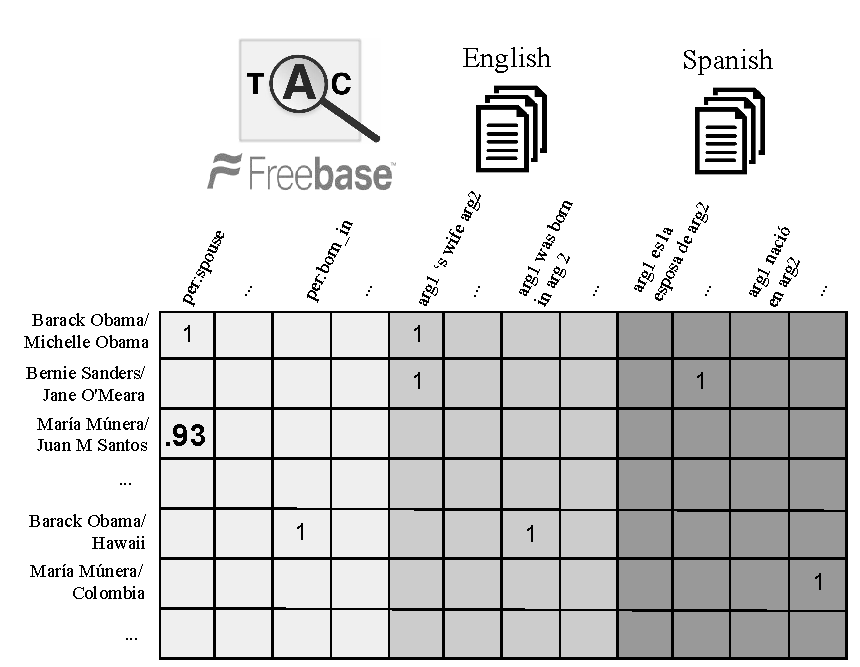
\includegraphics[scale=.68]{matrix}
\end{figure}

\begin{figure}[h]
\caption{Aggragating relation type vectors to form entity pair vector}
\centering
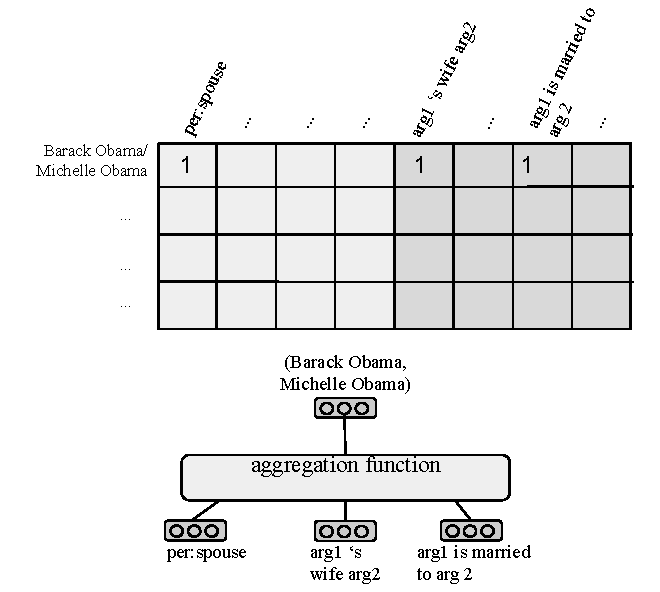
\includegraphics[scale=.68]{aggregate-entity}
\end{figure}


\subsection {Aggregation Functions}
\begin{itemize}
  \item Mean Relation : average all relation-type vectors for a given entity pair
  \item Max Relation :
  \item TopK Relations :
  \item Dimension-wise Max Pool :
  \item Convolution + Dimension-wise Max Pool :
\end{itemize}